\chapter{Desenvolvimento}

\section{Dispositivos utilizados}

\subsection{BeagleBone Black e OSSO Cape}

A BeagleBone Black é uma placa de desenvolvimento \textit{open-source}, desenvolvida pela \textit{Texas Instruments}, do tamanho aproximado de um cartão de crédito. Embora possua um tamanho diminuto, seu hardware é competente o suficiente para permitir rodar distribuições de \textit{Linux} como o Debian (a escolhida para esse projeto).

\begin{figure}[H]
        \begin{center}
                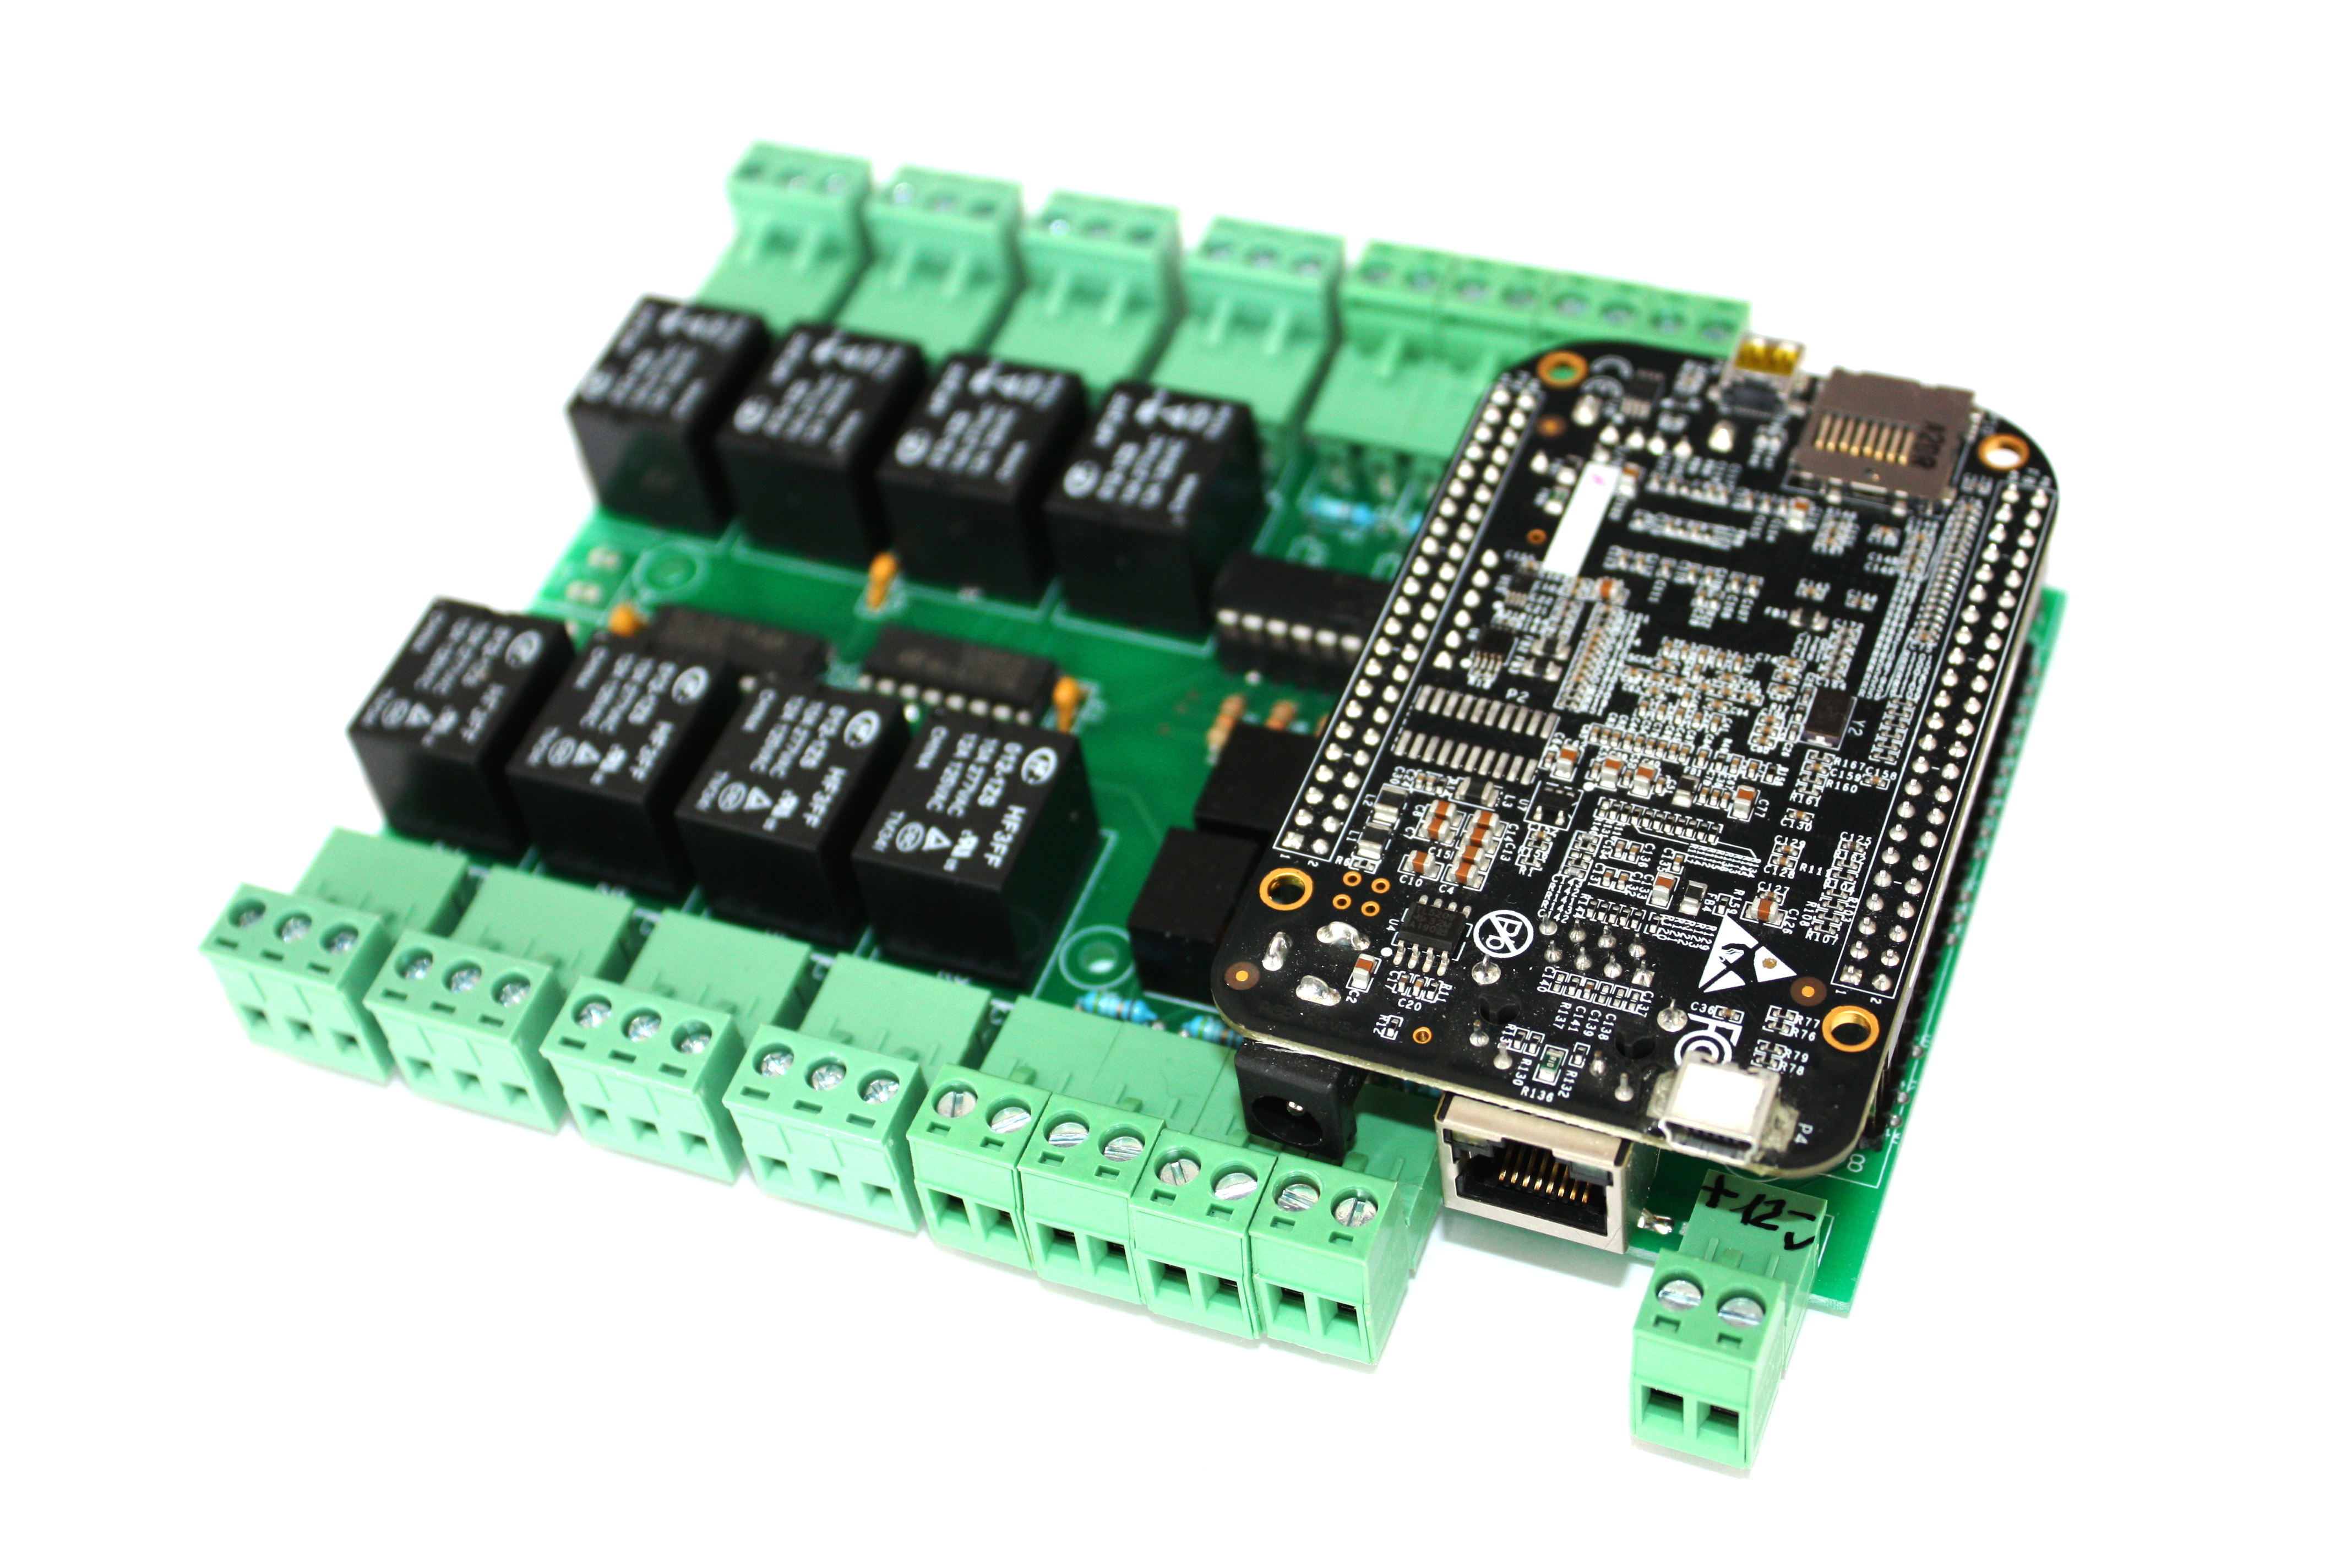
\includegraphics[width=0.8\textwidth,natwidth=585,natheight=180]{assets/images/devices-beaglebone.jpg}
                \caption{BeagleBone Black e OSSO Cape}
                \label{fig:bbb}
        \end{center}
\end{figure}

A BeagleBone permite expansões por meio \textit{capes}, placas não-oficiais que permitem melhor explorar o uso das saídas e entradas. Nesse projeto, foi utilizada a OSSO Cape, sendo que os seguintes recursos facilitaram a implementação do protótipo:

\begin{itemize}
  \item Oito entradas digitais optoacopladas
  \item Oito saídas digitais por meio de relês
  \item Saída RS-485 integrada
  \item Gerenciamento de fontes externas com tensões entre 5 à 24V
\end{itemize}

\subsection{Medidor de Energia Kron Mult-K}

O medidor de energia é essencial para informar tanto ao usuário, quanto ao sistema central, quanta energia foi consumida durante o período do carregamento. O dispositivo escolhido foi o Kron Mult-K, pois esse permite a medição de energia consumida sem a utilização de TCs e os dados são disponibilizados via MODBUS-RTU (conexão RS-485).

\begin{figure}[H]
        \begin{center}
                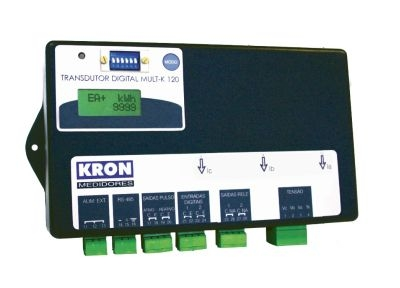
\includegraphics[width=0.8\textwidth,natwidth=400,natheight=288]{assets/images/devices-kron.jpg}
                \caption{Medidor Kron da série Mult-K}
                \label{fig:bbb}
        \end{center}
\end{figure}

\subsection{Phoenix EM-CP-PP-ETH Controller}

Os padrões de carregamento rápido utilizam protocolo de comunicação entre carro e estação e, visto a complexidade de decodificar e codificar tais protocolos, foi escolhido utilizar um controlador externo. O Phoenix EM-CP-PP-ETH permite gerenciar carregamentos AC, utilizando três fases em sua alimentação, e realizar todo controle necessário para o sequenciamento de inicialização e finalização de carregamentos.

\subsection{IHM WEG MT}

Para o usuário utilizar a EVSE, é necessária uma interface que apresente as informações necessárias e, além disso, seja robusta a intempéries como calor excessivo e chuva. Para tal, foi escolhida uma \ac{IHM} da WEG.

Utilizando o \textit{software EasyBuilder 8000}, é possível definir as telas que serão utilizadas pelo usuário, assim como os dados que serão exibidos. Os dados e o controle da IHM são dados por meio de diversos protocolos, dentre eles o MODBUS-TCP, o qual foi escolhido para o projeto.

\begin{figure}[H]
        \begin{center}
                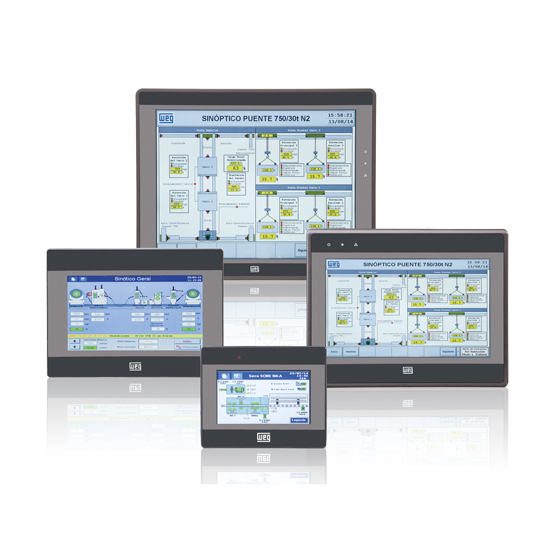
\includegraphics[width=0.8\textwidth,natwidth=400,natheight=288]{assets/images/devices-hmi.jpg}
                \caption{Linha de IHMs MT da WEG}
                \label{fig:bbb}
        \end{center}
\end{figure}

\section{Implementação do Projeto}

\begin{figure}[H]
        \begin{center}
                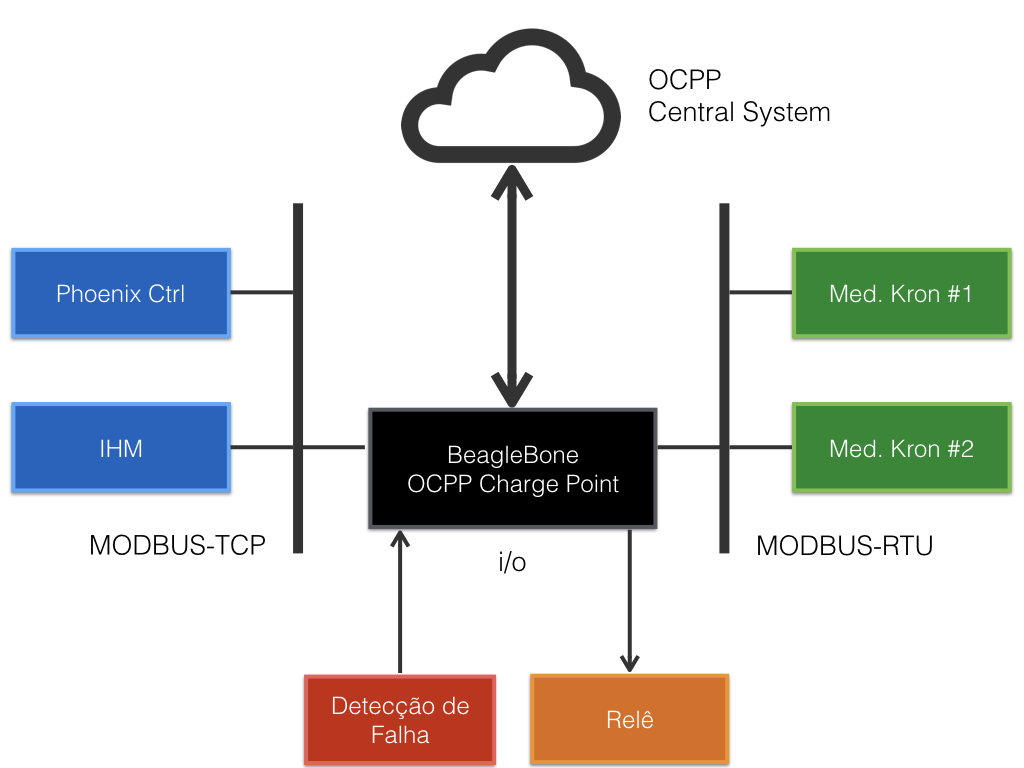
\includegraphics[width=0.8\textwidth,natwidth=400,natheight=288]{assets/images/devices-diagram.png}
                \caption{Diagrama de conexão entre os dispositivos da EVSE}
                \label{fig:proj-diagram}
        \end{center}
\end{figure}

A figura \ref{fig:proj-diagram} apresenta o diagrama de conexão dos dispositivos. Como todos os dispositivos são compatíveis com MODBUS, esse foi o protocolo escolhido para a comunicação entre eles. Para a comunicação entre servidor e estação, foi escolhido o protocolo \ac{OCPP}.

A estação possui dois medidores, sendo um de carregamento normal/lento e outro de carregamento rápido. Cada conector possui seu próprio medidores de energia, porém seus controles se dão de forma diferente: o de carregamento rápido utiliza o controlador Phoenix, enquanto o conector normal é controlado pela \textit{BeagleBone} e um relê, visto que ele é somente uma tomada comum e não necessita de nada muito elaborado para inicializar carregamentos (diferente do rápido, onde há um protocolo entre estação e carro).

\subsection{Comunicação MODBUS entre periféricos}



\subsection{Comunicação OCPP}
\subsection{Modificações Linux}
\subsection{Desenvolvimento de telas e sistema central}
\subsection{Funcionamento do Software}

\section{Testes}

\subsection{Ferramentas de teste}
\subsection{Testes iniciais}
\subsection{Testes na estação protótipo}
